\documentclass[11pt,a4paper]{article}
\usepackage[margin=1in]{geometry}
\usepackage[utf8]{inputenc}
\usepackage{amsmath,amssymb}
\usepackage{booktabs}
\usepackage{xcolor}
\usepackage{hyperref}
\usepackage{enumitem}
\usepackage{titlesec}
\usepackage{tcolorbox}
\usepackage{tikz}
\usetikzlibrary{shapes.geometric, arrows, positioning}

\hypersetup{
    colorlinks=true,
    linkcolor=blue!70!black,
    citecolor=blue!70!black,
    urlcolor=blue!70!black
}

\titleformat{\section}{\large\bfseries\color{blue!70!black}}{\thesection}{1em}{}[\titlerule]
\titleformat{\subsection}{\normalsize\bfseries\color{black!85}}{\thesubsection}{1em}{}

\title{
    \vspace{-1.5cm}
    \textbf{\Large Final Year Capstone Project Proposal \& Progress Report}\\[0.3cm]
    \textbf{\LARGE PARISCV v2: Fast Cycle-Accurate Microarchitectural Modeling and Custom Instruction Discovery for OpenHW RISC-V Processors}\\[0.2cm]
    \large Target Conference: IEEE HiPC 2026 Student Research Symposium (SRS)
}
\author{
    \textbf{Student Name:} Kushal R \quad | \quad \textbf{Department:} Computer Science \& Engineering\\
    \textbf{Project Advisor:} Faculty Advisor Name \quad | \quad \textbf{Co-Investigator:} Senior Collaborator Name\\
    \textbf{Academic Year:} 2026--2027
}
\date{\today}

\begin{document}

\maketitle

\begin{tcolorbox}[colback=blue!5!white,colframe=blue!70!black,title=\textbf{Executive Summary}]
This capstone project presents \textbf{PARISCV v2}, an automated framework for rapid microarchitectural performance modeling, ISA extension prediction, and custom instruction discovery on OpenHW RISC-V processors (CV32E40X with CV-X-IF and CV32E40P). By driving a calibrated 4-stage pipeline timing model directly from Spike ISS traces, the framework predicts real-core cycle counts in seconds. 
\begin{itemize}[leftmargin=*,noitemsep]
    \item \textbf{Phase 1 (Completed):} Validated cycle model across 14 Embench-IoT points against Verilator RTL simulation (0.00\%--3.45\% error bound), pre-RTL extension prediction (Zbb, Xpulp), and native custom instruction verification.
    \item \textbf{Phase 2 (Proposed Extension):} Expanding the framework with coarse-grained sub-word SIMD acceleration for Edge-AI (\textbf{TinyML} 4$\times$INT8 dot products over CV-X-IF) and automated \textbf{PPA (Power, Performance, Area)} Pareto optimization using open-source logic synthesis (Yosys + Sky130).
\end{itemize}
\end{tcolorbox}

\section{Introduction \& Problem Statement}
Exploring custom instruction extensions and processor configurations currently presents a fundamental dilemma in computer architecture:
\begin{enumerate}[leftmargin=*]
    \item \textbf{RTL Simulation Bottleneck:} Full Register-Transfer Level (RTL) simulation on Verilator or FPGA provides exact ground truth but requires hours to days per benchmark sweep, making early-stage Design Space Exploration (DSE) prohibitive.
    \item \textbf{Instruction Simulators Lack Timing:} Fast Instruction Set Simulators (ISS) like Spike execute millions of instructions per second but omit pipeline stalls, branch flushes, and data hazards.
    \item \textbf{Coprocessor Offload Latency:} Standard core interfaces (OpenHW CV-X-IF) introduce a 2-cycle offload and writeback handshake overhead. As a result, fine-grained scalar instruction fusion yields \textbf{0\% net speedup}, necessitating coarse-grained multi-operation acceleration.
\end{enumerate}

\noindent\textbf{Project Objective:} To develop a fast, calibrated cycle-accurate profiler that evaluates hardware choices in seconds without running RTL, and to leverage this engine to discover and synthesize optimal coprocessor instructions for modern embedded workloads.

\section{Phase 1: Completed Baseline Work (The Validated Profiler)}
The core profiling and validation engine is fully implemented and tested:

\subsection{Spike Trace Ingestion \& Microarchitectural Modeling}
\begin{itemize}[leftmargin=*]
    \item \textbf{Dynamic Register Reconstruction:} Replays commit logs (\texttt{spike --log-commits}) to recover exact divisors for multi-cycle arithmetic ($3 + \text{CLZ}$ cycles).
    \item \textbf{4-Stage Pipeline Stall Decomposition:} Analyzes compute cycles (IPC=1 baseline), branch flushes (3 cycles), jump flushes (2 cycles), target misalignment (+1 cycle on non-word-aligned 32-bit targets), and RAW load-use / \texttt{jalr} data hazards.
\end{itemize}

\subsection{Ground-Truth RTL Validation on Real OpenHW Cores}
The cycle model was validated against real Verilator simulations of \textbf{CV32E40X} and \textbf{CV32E40P} across 7 Embench-IoT kernels, with binary code layouts strictly pinned.

\begin{table}[h]
\centering
\small
\caption{PARISCV v2 Cycle Model Accuracy vs. Real Verilator RTL Simulation}
\label{tab:validation}
\begin{tabular}{lrrrrr}
\toprule
\textbf{Benchmark} & \textbf{Instructions} & \textbf{Model Cycles} & \textbf{RTL Cycles (40X)} & \textbf{Model Error} & \textbf{RTL Cycles (40P)} \\
\midrule
\texttt{matmult-int} & 97,748    & 134,546   & 134,545   & \textbf{+0.00\%} & 134,547 \\
\texttt{primecount}  & 2,273,871 & 3,927,267 & 3,927,224 & \textbf{+0.00\%} & 3,927,226 \\
\texttt{edn}         & 49,365    & 65,190    & 65,179    & \textbf{+0.02\%} & 65,181 \\
\texttt{tarfind}     & 53,846    & 118,587   & 117,149   & \textbf{+1.23\%} & 117,151 \\
\texttt{md5sum}      & 52,607    & 72,497    & 71,400    & \textbf{+1.54\%} & 71,402 \\
\texttt{statemate}   & 1,159     & 1,639     & 1,606     & \textbf{+2.05\%} & 1,608 \\
\texttt{crc32}       & 24,608    & 30,764    & 29,737    & \textbf{+3.45\%} & 29,739 \\
\bottomrule
\end{tabular}
\end{table}

\subsection{Key Phase 1 Outcomes}
\begin{enumerate}[leftmargin=*]
    \item \textbf{Pre-Synthesis Prediction:} Accurately predicted enabling Zbb bitmanipulation on CV32E40X within \textbf{--2.7\%} and Xpulp hardware loops on CV32E40P within \textbf{--0.10\%} before building RTL.
    \item \textbf{Native Decoder Instructions:} Discovered and verified in-pipeline custom instructions (\texttt{pg.idx}, \texttt{pg.rol}, \texttt{pg.sha}) saving up to 2,048 cycles.
    \item \textbf{The CV-X-IF Offload Finding:} Demonstrated that fine-grained scalar fusion (\texttt{pg.mac}) over CV-X-IF yields 0\% speedup due to interface round-trips, proving that coprocessor offloading requires multi-operation coarse-grained instructions.
\end{enumerate}

\newpage

\section{Phase 2: Proposed Project Extensions}

\begin{figure}[h]
\centering
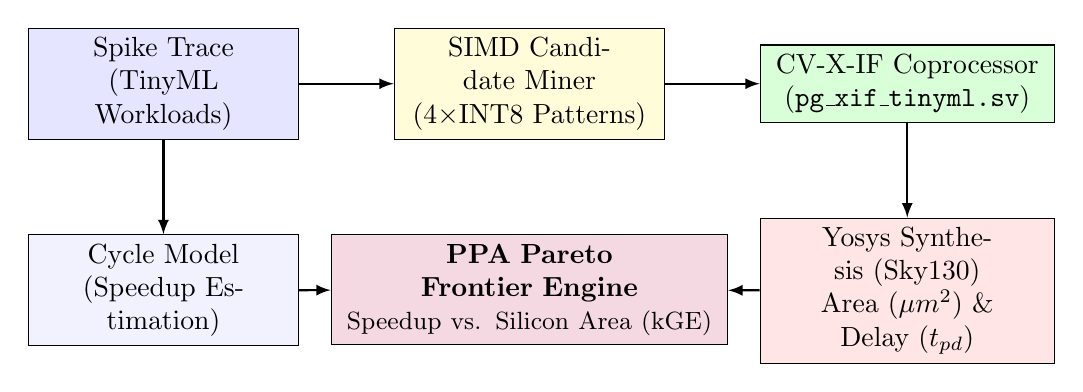
\begin{tikzpicture}[node distance=1.4cm, auto, >=latex]
    \node [draw, rectangle, fill=blue!10, text width=3.2cm, text centered] (trace) {Spike Trace\\(TinyML Workloads)};
    \node [draw, rectangle, fill=yellow!15, text width=3.2cm, text centered, right=1.2cm of trace] (miner) {SIMD Candidate Miner\\(4$\times$INT8 Patterns)};
    \node [draw, rectangle, fill=green!15, text width=3.5cm, text centered, right=1.2cm of miner] (rtl) {CV-X-IF Coprocessor\\(\texttt{pg\_xif\_tinyml.sv})};
    
    \node [draw, rectangle, fill=blue!5, text width=3.2cm, text centered, below=1.2cm of trace] (model) {Cycle Model\\(Speedup Estimation)};
    \node [draw, rectangle, fill=red!10, text width=3.5cm, text centered, below=1.2cm of rtl] (yosys) {Yosys Synthesis (Sky130)\\Area ($\mu m^2$) \& Delay ($t_{pd}$)};
    
    \node [draw, rectangle, fill=purple!15, text width=4.8cm, text centered, below=1.2cm of miner] (pareto) {\textbf{PPA Pareto Frontier Engine}\\\small Speedup vs. Silicon Area (kGE)};
    
    \draw [->, thick] (trace) -- (miner);
    \draw [->, thick] (miner) -- (rtl);
    \draw [->, thick] (trace) -- (model);
    \draw [->, thick] (rtl) -- (yosys);
    \draw [->, thick] (model) -- (pareto);
    \draw [->, thick] (yosys) -- (pareto);
\end{tikzpicture}
\caption{Phase 2 Architecture: Extending the cycle model with TinyML coprocessor acceleration and automated Yosys PPA Pareto exploration.}
\label{fig:phase2_arch}
\end{figure}

\subsection{Part A: Coarse-Grained Sub-Word SIMD for TinyML}
Building directly on the Phase 1 finding that CV-X-IF requires coarse-grained offloads, we target quantized INT8 Deep Learning kernels (INT8 GEMM, 2D Convolution, Depthwise Separable Conv):
\begin{itemize}[leftmargin=*]
    \item \textbf{The Baseline Bottleneck:} Executing a 4-element INT8 dot product on standard RV32IMC requires unpacking bytes with masks and shifts, 4 scalar multiplications, and 3 additions (16+ instructions, 16--20 cycles).
    \item \textbf{Coprocessor Acceleration (\texttt{pg.sdot4}):} We design \texttt{rtl/pg\_xif\_tinyml.sv}, a CV-X-IF coprocessor executing $(A_0 B_0 + A_1 B_1 + A_2 B_2 + A_3 B_3) + Acc$ in parallel via a 4-lane hardware multiplier-adder tree in \textbf{2 cycles total} (including bus handshake), achieving a projected \textbf{3.5$\times$--5.0$\times$ speedup}.
\end{itemize}

\subsection{Part B: Automated PPA (Power, Performance, Area) Exploration}
To extend cycle estimation into complete silicon feasibility:
\begin{itemize}[leftmargin=*]
    \item \textbf{Headless Yosys Synthesis:} A Python automation module generates Verilog datapaths for discovered candidates and executes headless synthesis against the open-source \textbf{SkyWater 130nm / Nangate 45nm} cell libraries.
    \item \textbf{Pareto Optimization:} Extracts silicon area ($\mu m^2$, Gate Equivalents) and critical path delay ($t_{pd}$) to generate \textbf{Speedup vs. Area (kGE) Pareto curves}, determining the most area-efficient coprocessor configurations.
\end{itemize}

\section{Project Roadmap \& HiPC 2026 SRS Target}

\begin{table}[h]
\centering
\small
\caption{Milestone Schedule}
\begin{tabular}{lll}
\toprule
\textbf{Milestone / Dates} & \textbf{Deliverable} & \textbf{Status} \\
\midrule
\textbf{Phase 1 (Completed)} & Calibrated Cycle Model (0.00\%--3.45\% err), Embench Validation & \textbf{Complete} \\
\textbf{Aug 23 -- Sep 24} & 2-Page Extended Abstract submission to \textbf{IEEE HiPC 2026 SRS} & \textbf{In Progress} \\
\textbf{Sep 25 -- Nov 15} & Implement \texttt{pg\_xif\_tinyml.sv} \& Yosys PPA Pareto Generator & Scheduled \\
\textbf{Dec 16 -- 19} & \textbf{Poster Presentation \& Lightning Talk at IEEE HiPC 2026 (Bengaluru)} & Target \\
\bottomrule
\end{tabular}
\end{table}

\section{Summary for Faculty Review}
\begin{itemize}[leftmargin=*]
    \item \textbf{Cycle-Accurate Profiler as the Core:} Phase 1 provides an already-functional, validated profiler with rigorous ground-truth evidence across 14 RTL data points.
    \item \textbf{High-Impact Phase 2 Additions:} Adding coarse-grained TinyML SIMD acceleration and automated Yosys PPA exploration addresses real-world chip design constraints.
    \item \textbf{Publication Track:} A complete 2-page extended abstract is prepared for peer-reviewed submission to IEEE HiPC 2026 SRS.
\end{itemize}

\end{document}
